% Chapter 4

\chapter{Dataset} % Main chapter title

\label{Chapter4} % For referencing the chapter elsewhere, use \ref{Chapter3} 

\lhead{Chapter 4. \emph{Dataset}} % This is for the header on each page - perhaps a shortened title

%----------------------------------------------------------------------------------------
\section{NIFTY 50}

The NIFTY 50 is the main index on the National Stock Exchange of India Ltd. (NSE). It tracks the performance of a selection of the biggest and most liquid Indian securities, including 50 of the approximately 1600 companies traded on NSE. This index covers around 65\% of the market's float-adjusted capitalization and is a good representation of the overall Indian stock market.
NIFTY 50 index covers a broad range of sectors in the Indian economy and provides investment managers with exposure to the Indian market in a single, efficient portfolio. It has been trading since 1996 and is ideal for benchmarking index funds and index-based derivatives. Using this index as the underlying asset, NIFTY index options were created.

\section{Data Collection}
\subsection{NIFTY Option Data}

\begin{figure}[htbp]
  \centering
    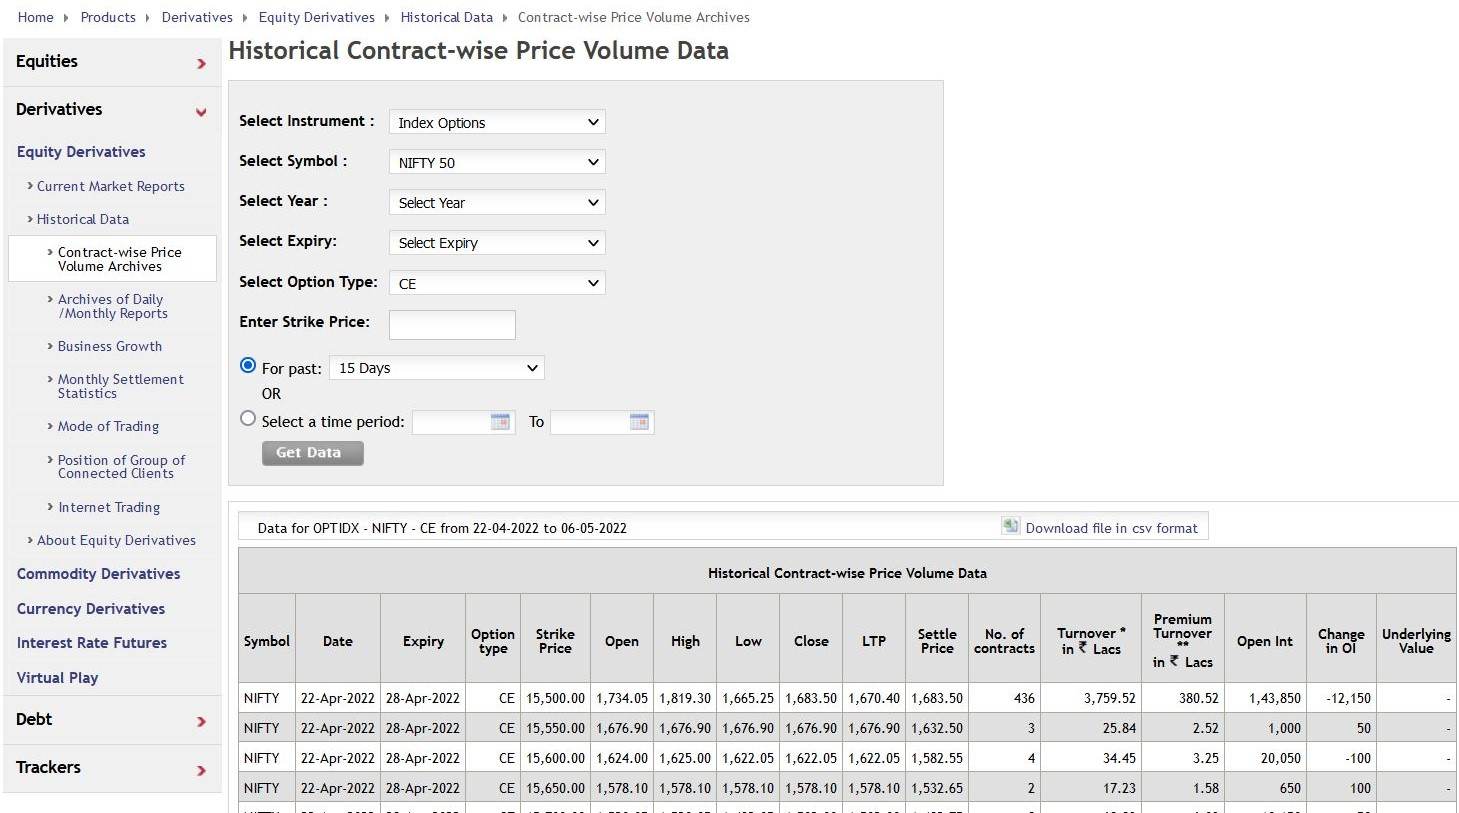
\includegraphics[scale=0.35]{Figures/data_collec_nifty_option.JPG}
    \rule{35em}{0.5pt}
  \caption[NIFTY Index Options]{NIFTY Index Options - Historical Data}
  \label{fig:data_collec_nifty_option}
\end{figure}

Data for NIFTY index options is available on the \href{https://www1.nseindia.com/products/content/derivatives/equities/historical_fo.htm}{NSE} website. The data used in this work contains information related to the NIFTY index put and call options between 2017 and 2022. Since the NSE website does not support scraping or downloading more than 90 consecutive days worth of data, data has been manually downloaded and combined for the target duration.
\\
\\

Figure ~\ref{fig:data_collec_nifty_option} shows a snapshot of the NSE website from which the option data has been downloaded.

\subsection{NIFTY Index Value}

Value of the underlying asset is an important piece of information for any derivative. While the option data contains a lot of information, the value of the underlying asset i.e. NIFTY index value, is not available for all the rows. To address this, the NIFTY index data for the same duration has also been downloaded from the \href{https://www1.nseindia.com/products/content/equities/indices/historical_index_data.htm}{NSE} webiste.

\begin{figure}[htbp]
  \centering
    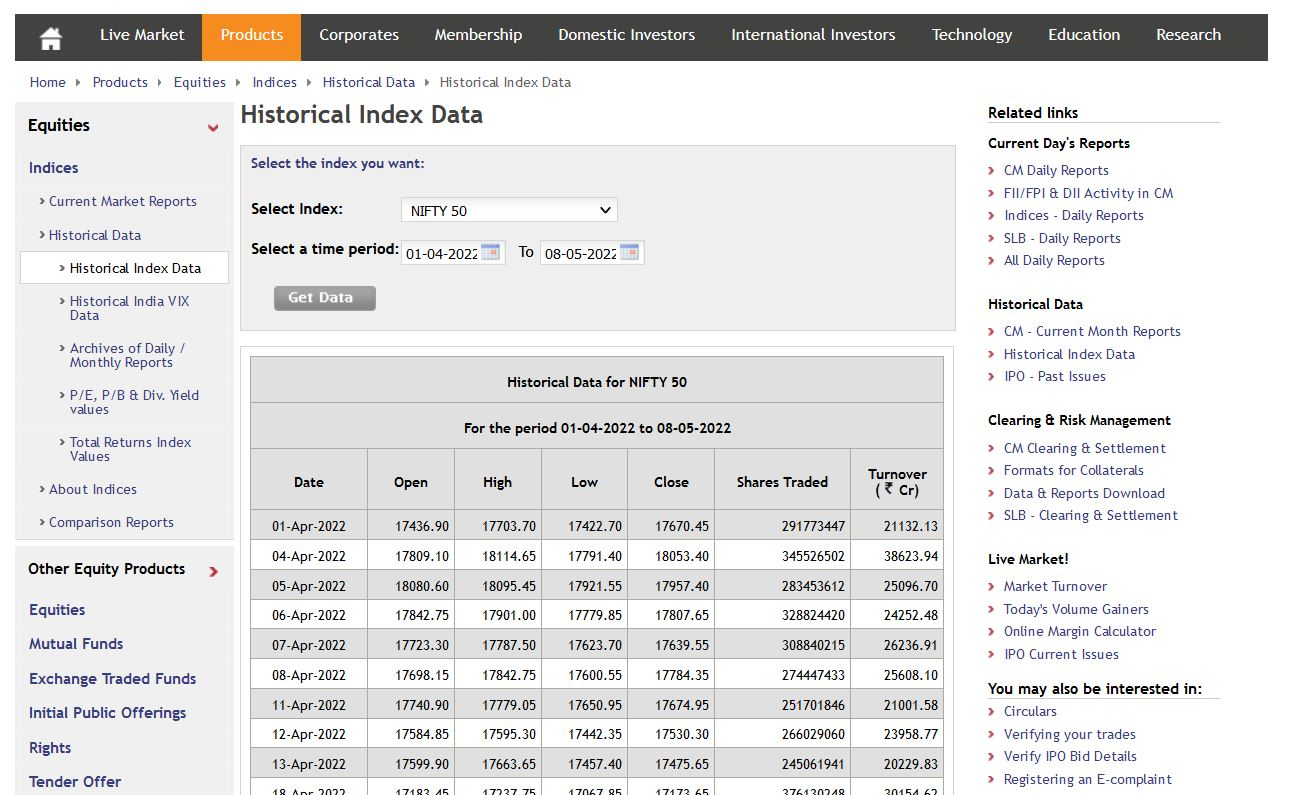
\includegraphics[scale=0.35]{Figures/data_collec_nifty_index.JPG}
    \rule{35em}{0.5pt}
  \caption[NIFTY Index Value]{NIFTY Index Value - Historical Data}
  \label{fig:data_collec_nifty_index}
\end{figure}

Figure ~\ref{fig:data_collec_nifty_index} shows a snapshot of the NSE website from which the index data has been downloaded.

\subsection{Risk Free Rate}

For risk free rate, yield of the 10 year government bond is used.   

\begin{figure}[htbp]
  \centering
    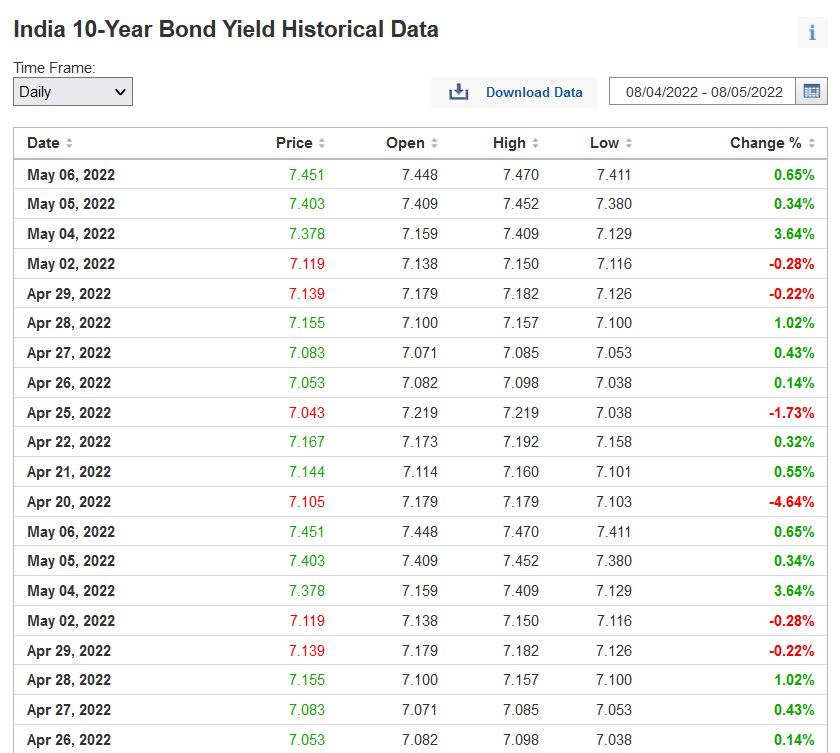
\includegraphics[scale=0.35]{Figures/data_collec_risk_rate.JPG}
    \rule{35em}{0.5pt}
  \caption[Risk Free Rate]{Risk Free Rate - Historical Data}
  \label{fig:data_collec_risk_rate}
\end{figure}

Figure ~\ref{fig:data_collec_risk_rate} shows past values of risk free rate in the context of Indian markets.

\section{Data Preparation}

Since all the data is currently in different CSV files, it needs be cleaned, prepared and merged to get the final data which will be used in the Neural Network and Black-Scholes model. Firstly, the duration needs to be calculated. To achieve this, we subtract the current date from the option expiry data and to normalize this duration, we divide it by 252, which is the number of trading days in a year. 

\begin{figure}[htbp]
  \centering
    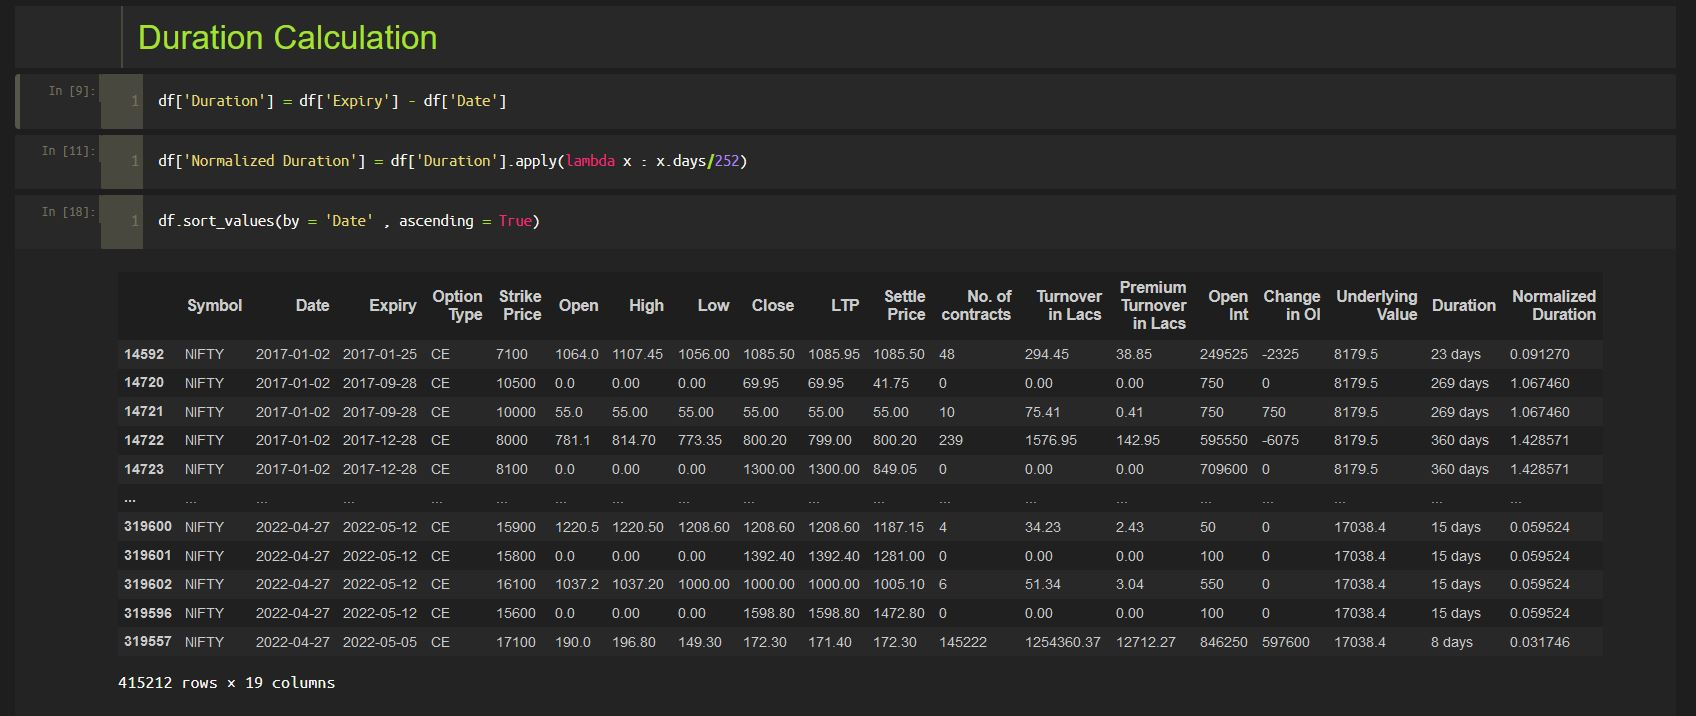
\includegraphics[scale=0.42]{Figures/data_prep_duration.JPG}
    \rule{35em}{0.5pt}
  \caption[Duration Calculation]{Duration}
  \label{fig:data_prep_duration}
\end{figure}

Apart from duration, volatility of the underlying asset is also an important feature for predicting the option premium. A 6 day window is chosen to calculate returns on the NIFTY index throughout each year. The standard deviation of this return for that particular year multiplied by $\sqrt{252}$ is used as historical volatility (sigma) in the models.

Figure ~\ref{fig:data_prep_volat} shows the code for calculating volatility. 

\begin{figure}[htbp]
  \centering
    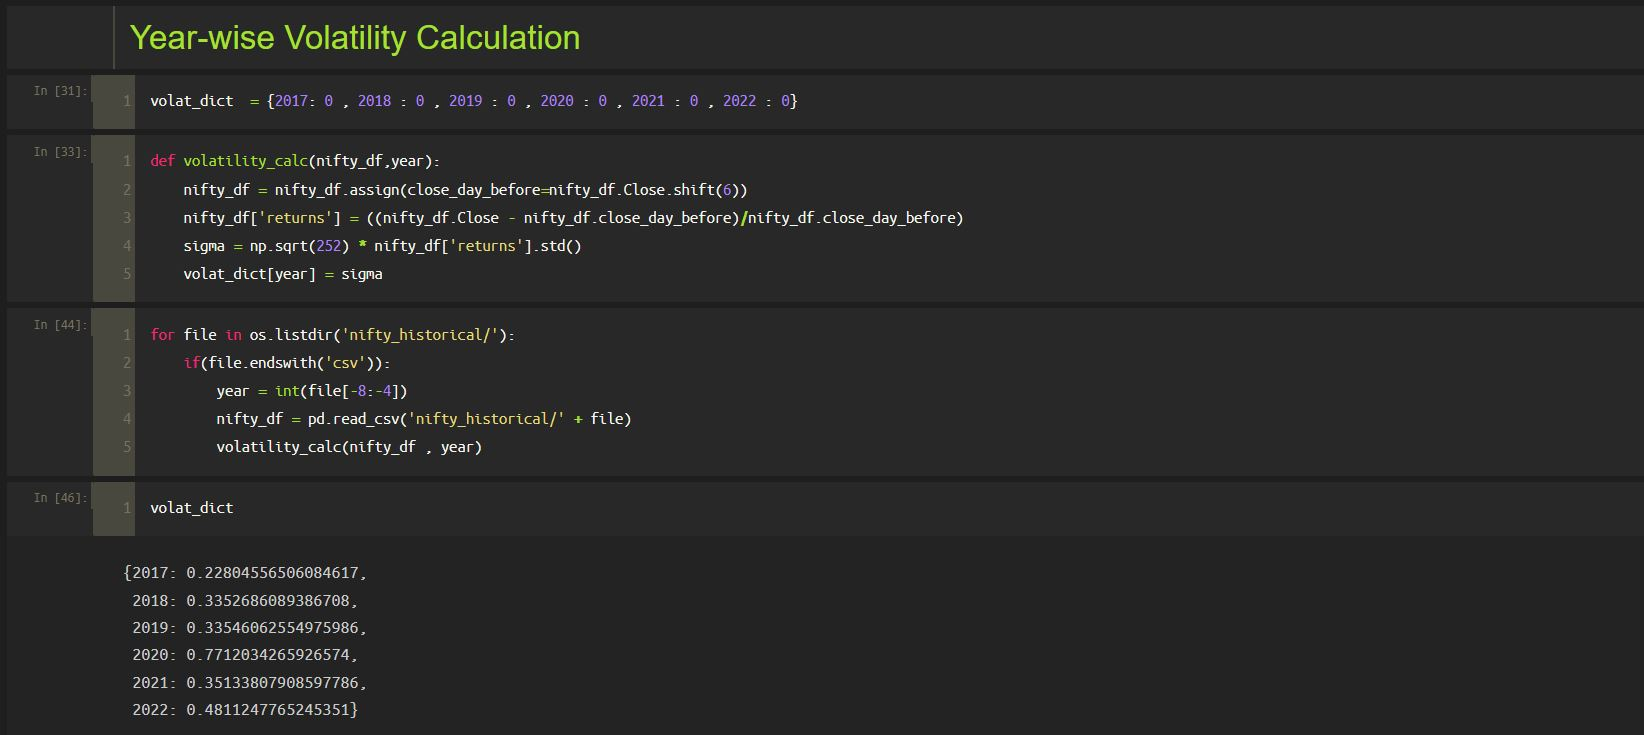
\includegraphics[scale=0.45]{Figures/data_prep_volat.JPG}
    \rule{35em}{0.5pt}
  \caption[Volatility Calculation]{Volatility}
  \label{fig:data_prep_volat}
\end{figure}

Finally, all this data is merged into one single dataframe which can be directly fed into the models.

\begin{figure}[htbp]
  \centering
    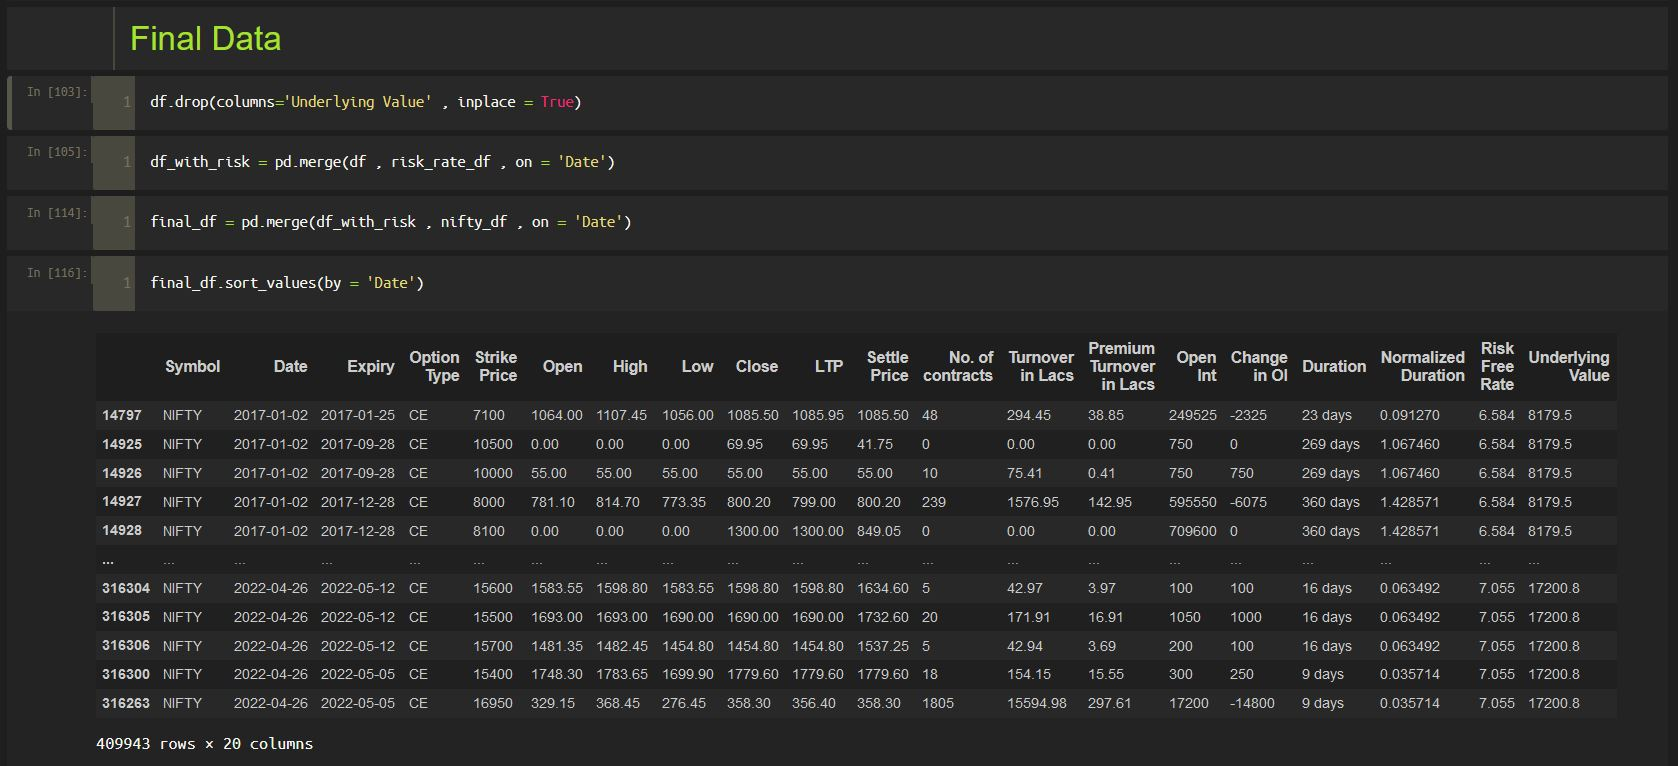
\includegraphics[scale=0.44]{Figures/data_prep_final.JPG}
    \rule{35em}{0.5pt}
  \caption[Final Data]{Final Data}
  \label{fig:data_prep_final}
\end{figure}

Figure ~\ref{fig:data_prep_final} shows the code for merging all the previous dataframes into the final dataframe. 

